% Introduction
\newpage

\section{Introduction}

\subsection{Problem Statement}

\subsubsection*{\underline{Context and Target Environment}}
The evolution of the "Smart Home" has transitioned from simple connectivity to the demand for intelligent automation. While the general market is saturated with fragmented IoT solutions, this project specifically targets modern urban households—such as mid-sized apartments or townhouses—occupied by busy families, elderly members, or pets. In these environments, standard smart platforms function merely as centralized remote controls. They enable manual actuation via smartphone applications but fail to deliver a cohesive, autonomous living experience tailored to the specific safety, convenience, and energy needs of an active urban family.

\subsubsection*{\underline{Key Challenges}}
Despite the ubiquity of connected hardware, several critical architectural and functional deficiencies persist in residential deployments:

\begin{itemize}
  \item \textbf{Data Silos \& Fragmentation:} Devices from different manufacturers often operate on proprietary protocols. This fragmentation prevents the aggregation of data into a single Unified Source of Truth, making holistic analytics and cross-device correlation impossible. \cite{nxp_matter_standard_2021}
  \item \textbf{Deterministic vs. Probabilistic Limitations:} Current systems rely on rigid, rule-based automation (e.g., "turn on lights at 6 PM"). They lack the probabilistic reasoning needed to adapt to dynamic human routines or distinguish between a human and a pet triggering a motion sensor.
  \item \textbf{Data Rich, Information Poor (DRIP):} IoT devices generate high-velocity telemetry daily. Without robust Data Engineering pipelines (ETL processes) to filter noise, users are overwhelmed with raw notifications rather than actionable insights regarding energy anomalies.
  \item \textbf{Reactive Operation \& Energy Inefficiency:} Systems operate reactively (e.g., cooling a room only after it gets hot). This lag degrades user comfort and leads to significant energy waste, as the system cannot pre-emptively optimize resources.
\end{itemize}

\subsubsection*{\underline{Operational Assumptions \& Constraints}}
To effectively address these challenges, the H.E.R.A system is designed with the following bounded parameters:

\begin{itemize}
  \item \textbf{Physical Scope:} The system is optimized for a medium-sized residential house with an estimated area of approximately 100--150 square meters. Instead of focusing on a single enclosed room, H.E.R.A is designed to support multiple household zones such as the living room, bedrooms, kitchen, and common areas. The spatial model therefore focuses on house-level environmental monitoring, zone-based device control, and resident interaction across the home while keeping the deployment scope realistic for a residential prototype.
  \item \textbf{Infrastructure Compatibility:} The architecture assumes the presence of a stable Wi-Fi network for cloud-based AI processing (such as NLP and heavy predictive modeling). However, it requires local Edge processing capabilities (e.g., via ESP32) to maintain critical deterministic operations and sensor readings if internet connectivity drops.
  \item \textbf{Privacy \& Security:} Given the continuous ingestion of environmental telemetry and voice commands, the system is constrained by strict data privacy requirements, ensuring that behavioral data and audio inputs are securely processed and shielded from unauthorized access.
\end{itemize}

\subsubsection*{\underline{The Need for a Solution and Scope of Intelligence}}
There is an urgent need for a comprehensive AIoT (AI + IoT) platform that bridges the gap between physical control and cognitive processing for urban homes. A truly intelligent system must transcend basic command execution to act as a proactive agent. H.E.R.A addresses this by narrowing its "smart" focus onto three prioritized pillars:

\begin{enumerate}
  \item \textbf{AI-Enhanced Security:} Utilizing machine learning to differentiate between genuine human presence and pets, thereby eliminating false alarms and providing reliable monitoring.
  \item \textbf{Proactive Energy Management:} Deploying predictive analytics to optimize power consumption based on historical usage patterns and environmental forecasts.
  \item \textbf{Frictionless Interaction:} Leveraging Natural Language Processing (NLP) to allow residents to control their environment intuitively, effectively shifting the paradigm from manual "Smart Control" to autonomous "Smart Living."
\end{enumerate}

% \subsection{Stakeholders of the Project}

% \subsubsection{Residents (Family Members)}
% Residents are the end-users who interact with the smart home environment daily. Their primary concern is comfort, convenience, and health.
% \begin{itemize}
%     \item \textbf{Pain Point:} They are tired of manually adjusting multiple apps for different devices and want a system that "just understands" their preferences.
%     \item \textbf{Benefit:} They gain a hands-free experience where the home adjusts temperature and lighting based on their presence and habits, along with health monitoring through air quality sensors.
% \end{itemize}

% \subsubsection{System's Administrator}
% The System's Administrator is the decision-maker responsible for the property's maintenance, security, and operational costs.
% \begin{itemize}
%     \item \textbf{Pain Point:} They struggle with rising electricity bills and the anxiety of potential security breaches or fire hazards when away from home.
%     \item \textbf{Benefit:} They receive detailed analytics on energy consumption to identify waste, along with real-time, AI-filtered security alerts that distinguish between false alarms (e.g., a pet) and genuine threats.
% \end{itemize}

\subsection{Stakeholders and Key Users}
To keep the project scope focused and consistent with the intended residential use case, the H.E.R.A system identifies only one core user group:

\begin{itemize}
  \item \textbf{Residents:} Residents are the primary and only target users of the system. They live in and interact with the smart home environment on a daily basis. Their main concerns include comfort, convenience, health protection, energy awareness, and household safety. They use H.E.R.A to monitor environmental conditions, issue voice or text commands, receive alerts, and control connected devices across the house.
\end{itemize}

% \subsection{Business Requirements}
% Derived from the analysis of Key Users, the project establishes the core business requirements that the H.E.R.A system must fulfill:

% \noindent \textbf{BR1: For Residents (Primary Key Users)}
% \begin{itemize}
%     \item Business Objective: To enhance the quality of life, convenience, and health protection through an automated living environment that proactively understands the user.
%     \item Pain Points: Users are fatigued by manually adjusting multiple applications for different devices; they desire a system that intuitively ``understands'' their preferences and routines.
%     \item Needs: A truly hands-free experience where the home autonomously adjusts temperature and lighting based on occupancy and habits, alongside health monitoring via environmental sensors.
%     \item Success Criteria: The system accurately processes unstructured language commands (via NLP) and autonomously executes environmental adjustments (e.g., lighting, HVAC) according to the context, completely eliminating the need for manual smartphone app interactions.
% \end{itemize}

% \noindent \textbf{BR2: For the System's Administrator (Secondary Key Users)}
% \begin{itemize}
%     \item Business Objective: To optimize operational costs (specifically electricity consumption) and ensure robust, reliable security for the property.
%     \item Pain Points: Persistent anxiety regarding rising electricity bills, potential security breaches, or fire hazards when away from home. Furthermore, the constant nuisance of false security alarms is a significant concern.
%     \item Needs: Detailed analytical reports on energy consumption to identify waste, coupled with real-time, AI-filtered security alerts that accurately distinguish between false alarms (e.g., a pet moving) and genuine threats.
%     \item Success Criteria: The provision of an interactive Dashboard displaying energy consumption metrics and forecasts; and the successful deployment of a Classification Model to differentiate human from pet movements, thereby significantly minimizing the rate of false alarm notifications.
% \end{itemize}

\subsection{Solution}
To fulfill the resident-centered business requirements, the H.E.R.A (Home Environment \& Response Assistant) is a comprehensive AI-powered virtual assistant system designed to improve daily residential living. Unlike traditional passive smart homes, H.E.R.A integrates a robust IoT infrastructure with advanced Natural Language Processing (NLP) and Data Analytics. This fusion allows the system to continuously monitor environmental conditions across a medium-sized house while also understanding and executing resident commands via voice or text. By bridging the gap between raw telemetry and human intent, H.E.R.A delivers a living environment that is proactively energy-efficient, secure, and deeply personalized for residents.

\subsubsection*{\underline{System Workflow}}
The system operates on a dual-stream data pipeline, integrating both automated environmental monitoring and user-centric interaction into a unified architecture:

\begin{enumerate}
  \item \textbf{Multi-modal Data Acquisition:}
    The system continuously ingests data from two primary sources:
    \begin{itemize}
      \item  Telemetry: Sensors monitor physical parameters (temperature, humidity, motion) and device states, transmitting data via MQTT.
      \item User Interaction: A dedicated interface captures voice commands or text inputs from the user, serving as the direct communication bridge.
    \end{itemize}

  \item \textbf{Processing \& Verification:}
    A centralized backend processes these incoming streams. For telemetry, it filters noise and verifies if data exceeds safety thresholds. Simultaneously, for user inputs, it initiates a Speech-to-Text (STT) process (if applicable) to convert audio signals into processable query strings.

  \item \textbf{Intelligence Layer (NLP \& Analytics):}
    This is the decision-making core:
    \begin{itemize}
      \item Natural Language Understanding (NLU): AI models analyze user queries to extract intents (e.g., "turn on") and entities (e.g., "living room light").
      \item Predictive Analytics: Machine learning algorithms analyze historical logs to forecast trends or detect anomalies, enriching the decision context.
    \end{itemize}

  \item \textbf{Action, Control \& Feedback:}
    Based on either AI interpretation or threshold triggers, the system executes commands:
    \begin{itemize}
      \item Device Control: Sending signals to microcontrollers (ESP32/YoLo) to adjust physical devices.
      \item User Response: Generating a natural language response (Text-to-Speech) to confirm actions or report status back to the user.
    \end{itemize}

  \item \textbf{Activity Logging:}
    Every interaction—whether a sensor reading, a voice command, or a system automated response—is recorded in an activity log. This maintains a single source of truth for debugging, dashboard visualization, and future model training.
\end{enumerate}

By combining reactive automation with interactive AI capabilities, this workflow fulfills the dual purpose of a robust monitoring system and an intelligent virtual assistant.

\subsubsection*{\underline{Architectural Hierarchy}}
To ensure scalability, maintainability, and a clear separation of concerns, the H.E.R.A system architecture is bifurcated into two distinct layers. This two-tier design decouples the physical hardware constraints from the high-level computational logic:

\begin{figure}[H]
  \centering
  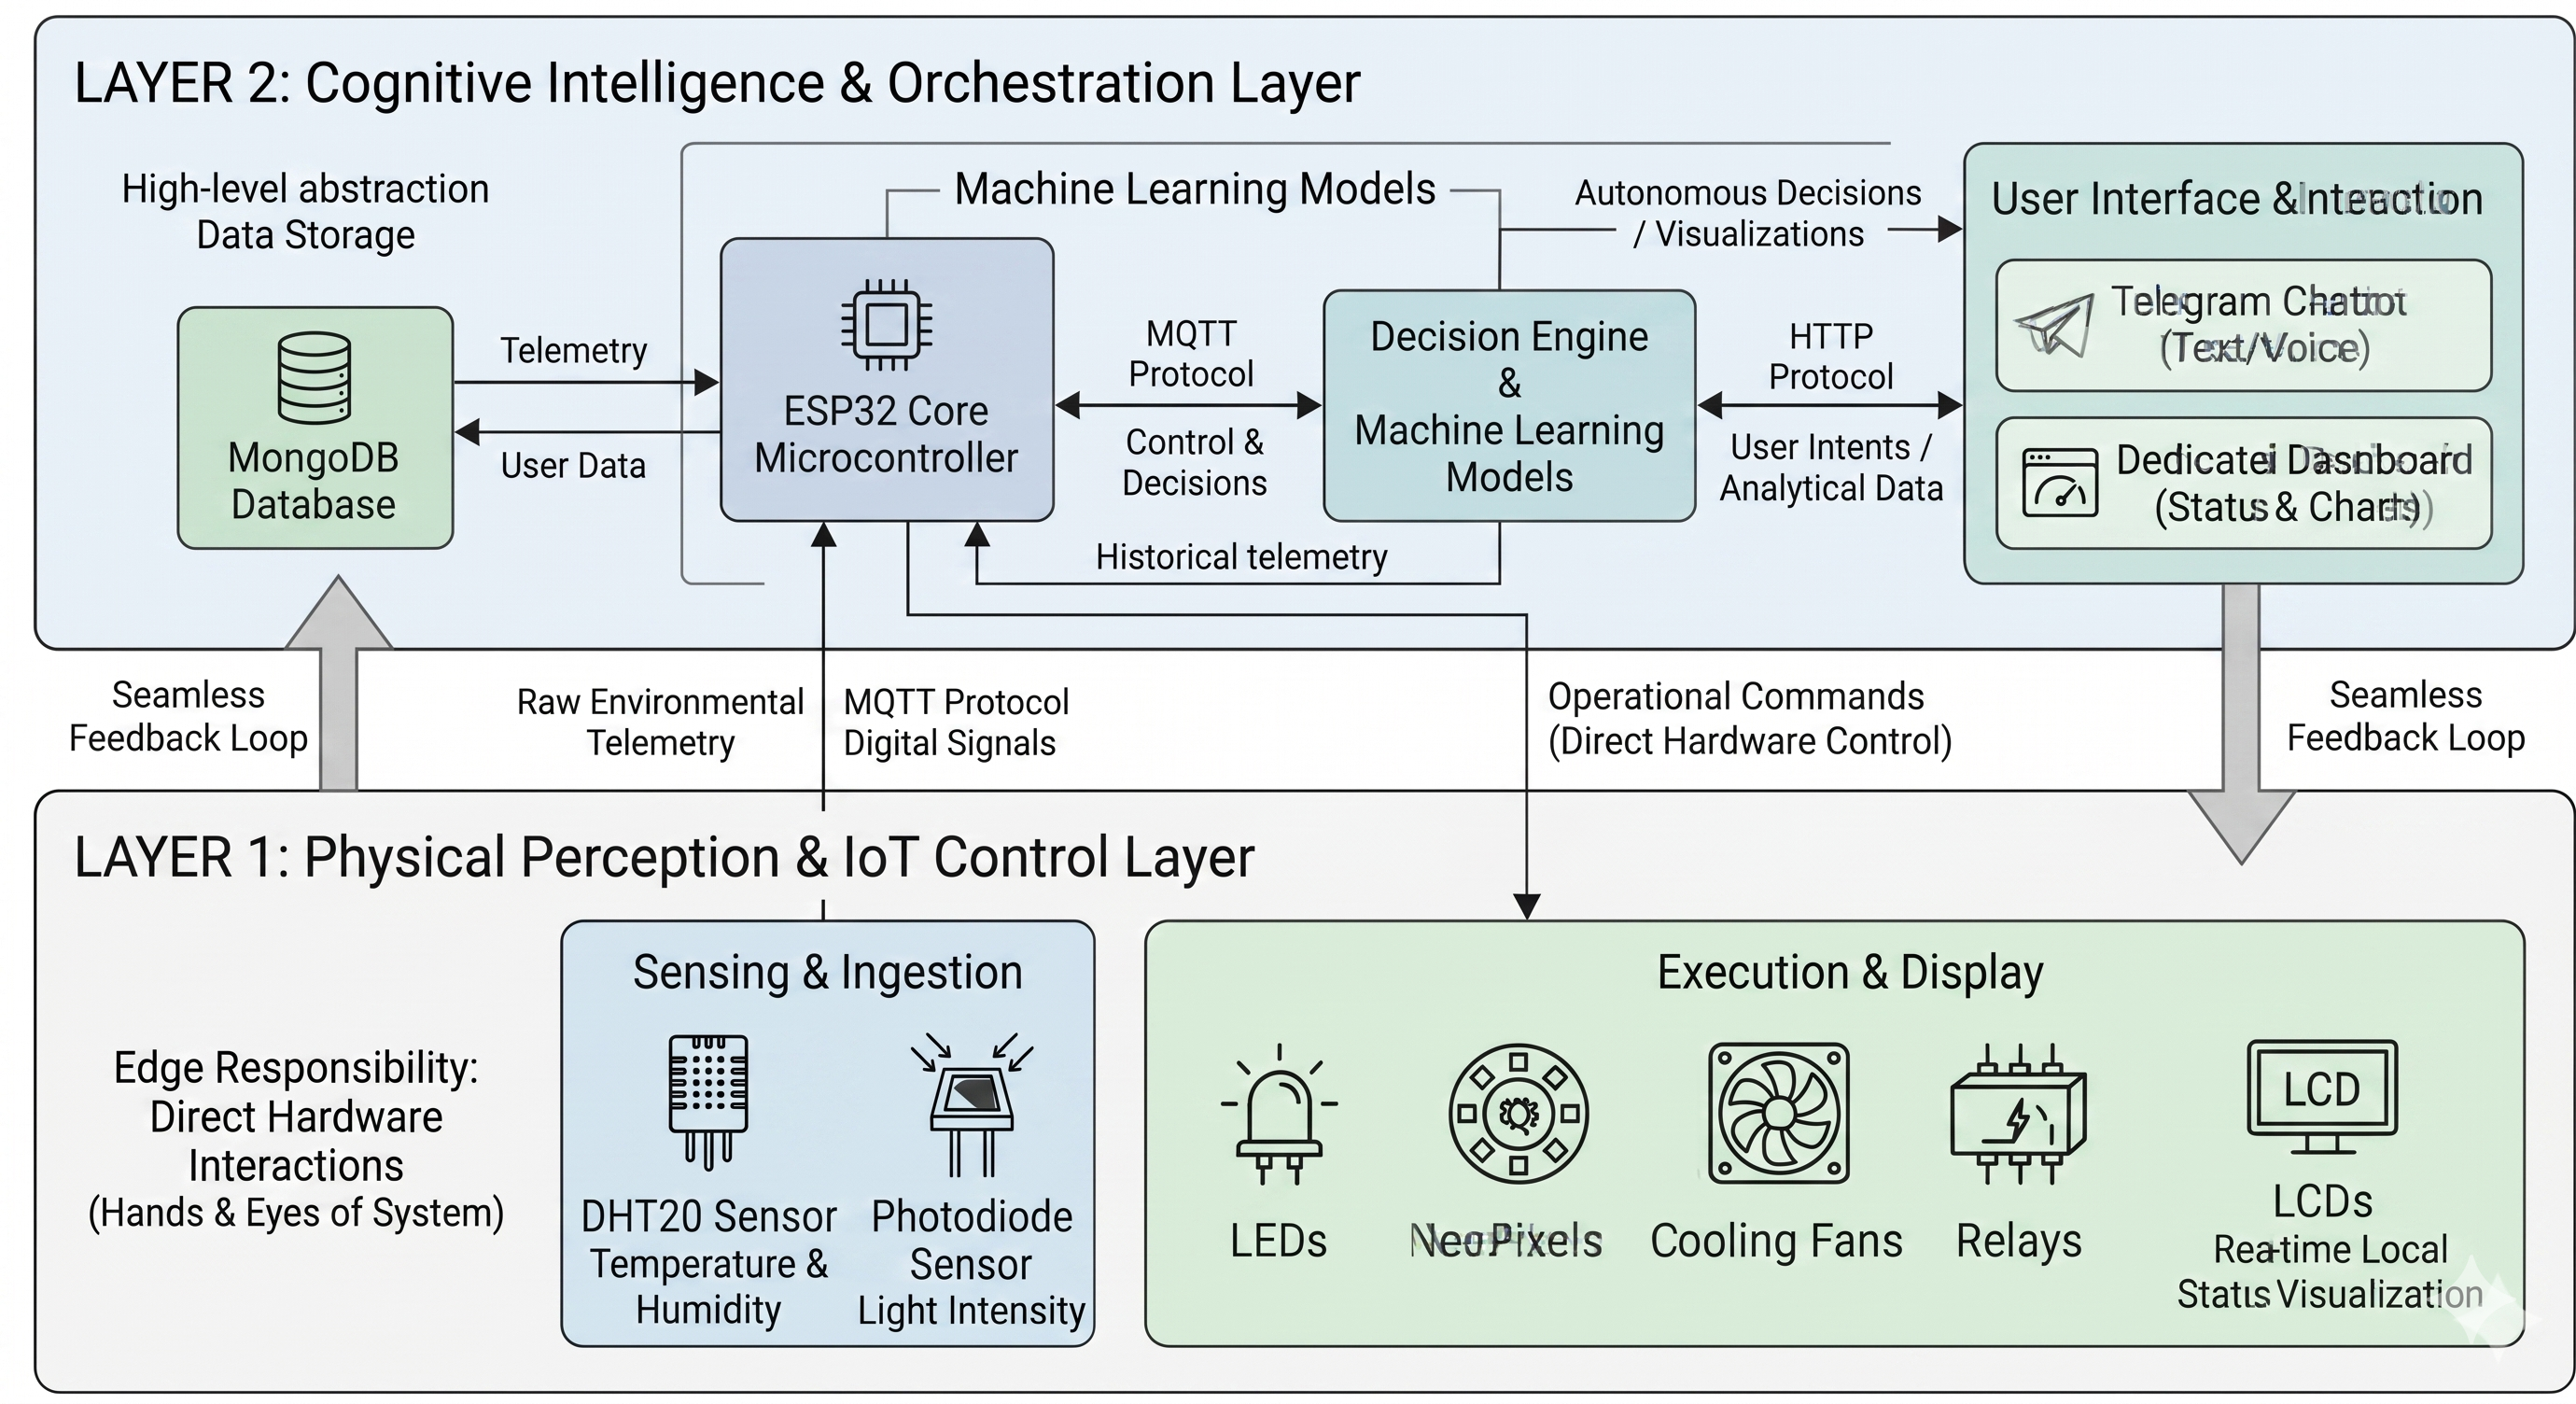
\includegraphics[width=1\textwidth]{image/system_architecture.png}
  \caption{System Architecture of H.E.R.A}
  \label{fig:system-architecture}
\end{figure}

\begin{itemize}
  \item \textbf{Layer 1: The Physical Perception \& IoT Control Layer} \\
    This foundational layer serves as the direct interface with the physical environment. It is responsible for Data Acquisition and Device Actuation.
    \begin{itemize}
      \item \textbf{Sensing \& Ingestion:} Utilizing the DHT20 sensor, this layer captures raw environmental telemetry (specifically temperature and humidity) and converts physical phenomena into digital signals. These signals are transmitted to the core processing unit via the lightweight MQTT protocol to ensure stable, low-latency communication.
      \item \textbf{Execution \& Display:} This component receives operational commands from the upper layer and executes them through various actuators—including LEDs, NeoPixels, cooling fans, and relays—to physically alter the home environment. Additionally, it utilizes LCDs for real-time local status visualization.
      \item \textbf{Edge Responsibility:} It handles immediate hardware interactions at the sensor/actuator level, acting as the reliable "hands and eyes" of the smart home system.
    \end{itemize}

  \item \textbf{Layer 2: The Cognitive Intelligence \& Orchestration Layer} \\
    Powered by an ESP32 core microcontroller acting as the main processing bridge and backed by a MongoDB database, this high-level layer abstracts the complexity of data storage, user interaction, and decision-making.
    \begin{itemize}
      \item \textbf{User Interaction \& Interface:} Users can seamlessly interact with the system using text or voice commands via a Telegram Chatbot, which communicates with the core system using the HTTP protocol. To enhance user familiarity, a dedicated Dashboard is provided to display real-time statuses and analytical charts.
      \item \textbf{Decision Engine \& Machine Learning:} Utilizing historical telemetry stored securely in MongoDB, this engine employs compact Machine Learning (ML) models to assist in autonomous decision-making and to generate the data visualizations presented on the dashboard interface.
      \item \textbf{Orchestration:} Acting as the central coordinator, it processes high-level ML decisions and user intents (parsed from the Telegram bot), translates them into specific hardware commands, and dispatches them down to the IoT layer via MQTT for immediate execution.
    \end{itemize}
\end{itemize}

The interaction between these two layers creates a seamless feedback loop: Layer 1 provides the physical context and executes actions via MQTT, while Layer 2 (accessible via HTTP through the chatbot) provides the intelligence, persistent data storage, and actionable decisions.

\subsubsection*{\underline{User Interface \& Interaction}}
To provide a comprehensive and intuitive user experience, H.E.R.A. features a modern web-based dashboard built with React. This unified frontend interface allows users to monitor real-time environmental telemetry, manually control actuators, and interact directly with the multi-agent AI pipeline in one centralized location

% caption: The H.E.R.A unified web dashboard featuring real-time telemetry, device control, and AI chat interface.

% \subsubsection{System \& Security Monitor (Automated/External)}
% This represents the technical backbone or potentially a third-party monitoring service that ensures system integrity.
% \begin{itemize}
%     \item \textbf{Pain Point:} Managing the uptime and security of dozens of connected IoT devices is complex and prone to cyber vulnerabilities.
%     \item \textbf{Benefit:} The system provides logs of network activity and device health, enabling predictive maintenance before hardware failure occurs.
% \end{itemize}

\subsection{Goal of the Project}

\underline{\textbf{Primary Objectives:}}
\begin{itemize}
  \item Develop a Scalable IoT Architecture: Build a system capable of handling concurrent connections from multiple sensor nodes with low latency.
  \item Implement Data-Driven Automation: Move beyond simple timers to behavior-based automation using machine learning algorithms.
  \item Optimize Energy Consumption: Provide visualization and forecasting tools that empower users to reduce their carbon footprint and electricity costs.
  \item Enhance Security with AI: Utilize computer vision and anomaly detection techniques to provide superior security coverage compared to traditional motion sensors.
\end{itemize}

\underline{\textbf{Scope of the Project:}}
\begin{itemize}
  \item IoT Core Infrastructure:
    Implementation of essential smart home management features including device provisioning (registration), state synchronization (on/off status), real-time command dispatching via MQTT, and role-based access control (RBAC) for family members.

  \item Data Pipeline Integration:
    Development of automated ETL (Extract, Transform, Load) pipelines to ingest high-frequency sensor telemetry, clean noise, and structure data for analytical processing.

  \item AI-Driven Insights:
    Leveraging machine learning models to transform raw data into intelligence:
    \begin{itemize}
      \item Regression Models: Forecasting energy consumption trends for the upcoming month.
      \item Classification Models: Distinguishing between human presence and pets to filter false security alarms.
      \item Clustering Algorithms: Grouping similar user activity patterns to recommend personalized automation schedules.
    \end{itemize}

  \item Visualization \& Reporting:
    Deployment of interactive dashboards featuring heatmaps (for room occupancy) and time-series charts to visualize historical environmental data and real-time system states.

  \item Digital Twin Integration \& Simulation-to-Reality (Sim2Real):
    \begin{itemize}
      \item Virtual Environment Replication: Development of a 3D digital twin of the home environment to synchronize and visualize the real-time status of IoT devices and environmental sensors.
      \item Scenario Simulation: Creating "What-if" scenarios, such as fire outbreaks, gas leaks, or security breaches, to validate the responsiveness and accuracy of the system's emergency protocols without risking physical assets.
      \item Sim2Real Framework: Ensuring that the control logic and AI models developed in the simulation can be seamlessly transitioned to physical hardware with minimal reconfiguration, facilitating robust testing and reducing the risk of equipment failure during deployment.
    \end{itemize}

  \item Hardware \& Architecture Scope: To establish precise physical boundaries and fulfill the required minimum number of input/output (I/O) interfaces, the system's hardware is distributed across two primary computational nodes:
    \begin{itemize}
      \item Input Sensors: Integrates a Temperature/Humidity Sensor and a Light Sensor to continuously capture multi-modal environmental telemetry.
      \item Output Actuators \& Displays: Utilizes an LCD screen for real-time state visualization, alongside physical actuators including LED lights, a Mini Fan, and a Relay module to execute environmental adjustments and simulate appliance control.
    \end{itemize}

  \item The Central Processing Node (PC): Serving as the cognitive intelligence hub (Layer 2), a computer system integrates a Microphone (Sound Sensor) as its primary input. This node is strictly dedicated to intensive audio acquisition and Speech-to-Text (STT) processing , subsequently feeding the Natural Language Understanding (NLU) pipeline before dispatching execution commands to the Edge Node via MQTT.
\end{itemize}
